\documentclass{report}

\usepackage{biblatex}
\addbibresource{../../../Resources/resources.bib}

\usepackage{graphicx}
\usepackage{tikz}
\usetikzlibrary{arrows}
\usetikzlibrary{quantikz}

\usepackage[normalem]{ulem}

\usepackage{physics}
\usepackage{amsthm}
\usepackage{amsfonts}

\usepackage{hyperref}
\usepackage[
  top=1in,
  bottom=1in,
  left=1.5in,
  right=1.5in,
]{geometry}

\newtheorem{definition}{Definition}
\newtheorem{corollary}{Corollary}
\newtheorem{theorem}{Theorem}
\newtheorem{problem}{Problem}
\newtheorem{lemma}{Lemma}

\DeclareMathOperator{\CNOT}{CNOT}

\title{Bridging Gates over Qubits}
\author{Seyed Sajad Kahani \\Supervisor: Prof. Dan Browne}
\date{\today}
\begin{document}
\maketitle

\tableofcontents

\begin{abstract}
  
\end{abstract}

\chapter{Introduction}

Quantum computation (QC) is an emerging field that aims to use quantum mechanics to solve problems that are intractable for classical computers. Since the earliest conceptualization of quantum computation~\cite{feynman1986}, it has been believed that quantum computers could revolutionize the way we solve problems, particularly those involving simulating nature. Over time, it has become clear that quantum computers have applications far beyond physical simulations. There are algorithms for search and traversing graphs, solving linear equations~\cite{montanaro2016}, and methods for machine learning and optimization~\cite{jordan2023}.

Despite significant efforts, we are still far from fully utilizing these algorithms. Our current hardware technology has not yet achieved the desired accuracy and number of qubits necessary for quantum computers to outperform classical computers in solving useful problems. The current situation is commonly referred to as the ``noisy intermediate scale quantum'' (NISQ) era~\cite{preskill2018}, characterized by restricted resources, including a limited number of qubits, constrained qubit connectivity, hardware-specific gate sets, and limited circuit depth due to noise \cite{cross2019}.

The restricted qubit resources and excessive noise susceptibility of NISQ devices necessitate optimal compilers to have any hope of useful near-term quantum computation. A huge amount of research has been conducted to tackle different aspects of the compilation problem, including qubit allocation \cite{itoko2019,siraichi2018,paler2019,zhang2021,li2019}, routing \cite{childs,zhou2020,itoko2019,cowtan2019,nash2020,kissinger2019} and gate synthesis \cite{shende2006,vatan2004,vatan2004a,shende2004,barenco1995,dawson2006}. These aspects are deeply intertwined and one may not distinguish between them, but all of them are in some sense a circuit transformation from a higher-level circuit (with fewer imposed constraints) to a lower-level circuit (with more imposed constraints) \cite{hundt2022}.

% TODO, resolve TODO in cites
% TODO, improve the information in the following paragraph
{ \color{blue} WILL BE REVISED
While the knowledge of classical compilation is adopted and the divergent points (no-cloning \cite[TODO]{} and reversibility \cite{shende2003}) are studied and addressed well, another important distinction has received less attention - the cost of SWAP operations. In classical circuit synthesis, SWAPs simply rearrange wires at negligible cost, compared to two-bit gates. But in the quantum realm, SWAP gates require double entangling \cite[TODO]{} interactions between qubits, making them the most expensive two-qubit quantum logic gates \cite[TODO]{}. 

Despite extensive research into minimizing the overall number of SWAP operations~\cite[TODO]{childs}, there is little work addressing the inherent cost of each SWAP gate. A few recent works have proposed techniques to reduce the cost of SWAP gates, such as embedding SWAPs within other 2-qubit gates in 2QAN compiler~\cite{lao2021}, or optimization of SWAP decompositions into CNOT gates~\cite{kissinger2019,nash2020}. In this work, we aim to address the primary usage of SWAP gates - enabling connectivity between non-adjacent qubits. We analyze the possibility of simplifications for different connectivity cases.

Here we define a problem called bridging that is to find a circuit that applies a two-qubit gate on two non-adjacent qubits. By utilizing the framework of~\cite{kissinger2019} and the extensive literature of network coding \cite[TODO]{} show that in the classical case, the cost of bridging over $n$ bits is $4n$ to $6n$ (upto a $O(1)$ constant). We also present a circuit that achieves the lower bounds. We then attempt to extend the results to the quantum regime, by presenting a circuit to bridge two-qubit gates with Schmidt number $2$ over $n$ with optimal number of CNOTs.

This advancement will lead to $33\%$ reduction in the cost of the most expensive two-qubit gate in many situations. To demonstrate the practicality of our results, we implement the algorithms and benchmark with application-oriented dataset of circuits.

The rest of this thesis is organized as follows. Chapter~\ref{chap:background} reviews the related works. In Chapter~\ref{chap:discussion}, we present the algorithms and prove their correctness and optimality for the classical and quantum cases. We implement the algorithms and benchmark against state-of-the-art techniques in Chapter~\ref{chap:implementation}. Finally, Chapter~\ref{chap:conclusion} concludes and discusses avenues for future work. }


\chapter{Background}\label{chap:background}

We should be concerned with two key findings from the literature review on quantum compilation. First, the way that they broke down the problem and the assumption they made to simplify the problem space and introducing some structure to that. On the other hand, is the alogrithms that they involve techniques from QC, graph theory and more.

Here we try to review both of these aspects to draw a big picture of our notion of quantum compilation and also to review the existing techniques related to our approach, like the special techniques for two-qubit gates.

\section{Quantum Compilation}
The term ``quantum compilation'' can refer to any process that transforms a higher-level description of a quantum algorithm into a lower-level description~\cite{hundt2022}. In the majority of works \cite{zulehner2018,childs,cross2022,sivarajah2021,qiskit2023,paler2021}, circuits are the description used and thereby the compilation is done by transforming a general quantum circuit into a circuit that is compatible with a specific hardware. Given that the problem of finding the most optimal circuit (with respect to a sense of complexity like depth or number of gates) is proven to be NP-hard \cite{siraichi2018}, the research primarily centers on deconstructing this problem into smaller components and devising techniques to effectively balance between the agility of the process and the quality of the solution. This mirrors the approach adopted in classical compilation \cite{allen2001}.

However, the clear structure for this breakdown has not been firmly established, with numerous diverse approaches in play. As such, our goal is to provide a comprehensive overview of the issue and identify common patterns in the existing literature. This overall picture will then serve as a reference point throughout the rest of this thesis. To achieve this overview, it's crucial to define \textbf{circuit transformation} as a process that preserves the essential meaning of the circuit, ensuring that the circuit's output remains consistent for any input before and after the transformation. Yet, this process alters the circuit to adhere to specific constraints or optimize it for particular goals.

Thus, \textbf{quantum compilation} in our essay will be a sequence of circuit transformations where each transformation either enforces a constraint or optimizes the circuit (where optimization itself can be perceived as a soft constraint). The primary constraints imposed upon the circuit arise from the characteristics of the hardware and are listed below:

\begin{itemize}
  \item \textbf{Gate set}: The set of gates physically available in the hardware.
  \item \textbf{Connectivity}: The connectivity between qubits in the hardware topology.
\end{itemize}
  
Furthermore, the optimizations that corresponds to different degrees various degrees of freedom (e.g., qubit assignments, choosing among equivalent subcircuits) can be applied. They are commonly pursuing these goals:

\begin{itemize}
  \item \textbf{Complexity reduction}: Reducing the number of gates or depth of the circuit.
  \item \textbf{Preparation for constraints}: Minimizing violation of the mentioned constraints before imposing them. 
  \item \textbf{Error mitigation}: The error of the circuit with respect to the hardware, especially in NISQ devices.
\end{itemize}

Quantum compilation frameworks mainly use a similar approach, they introduce transformations that are each is somehow seeking one of the goals defined before, tket even uses the term predicates for the constraints that are similar to these \cite{sivarajah2021}. Typical transformations in their compilation process are, decomposing gates (imposing gate set constraint), assigning qubits (optimization of connectivity as a soft constraint), routing (imposing connectivity constraint), and further optimizations (reducing complexity). Yet the order of these transformations is not the same everywhere, for example, some \cite{lao2021,qiskit2023} deffer the gate synthesis after the routing while some \cite{wille2020,sivarajah2021} does it otherwise.

With this background established, we now dive into details on gate set and connectivity constraints, and circuit optimizations techniques for reducing complexity.

\subsection{Gate synthesis}

Imposing the gate set constraints which is known as the gate synthesis, is one of the oldest subroutines in the quantum compilation. The problem here is to decompose a general $n$-qubit gate into a sequence of gates from the physically available gates on the device. Here we review the results for the synthesis of one, two, and more than two-qubit gates. 

While most of the devices have the capability to perform arbitrary one-qubit gates, with a neglectible cost, there is a famous result for the synthesis of one-qubit gates, called Solovay-Kitaev theorem \cite{dawson2006}. It states that any one-qubit gate can be approximated by a sequence of gates from a universal gate set with an error of $\epsilon$ using $O(\log^c(1/\epsilon))$ gates, where $c$ is a constant. Here as like as other results, we assume that all of one-qubit gates are available.

For two-qubit gates, it is known that the set of all one-qubit gates together with CNOT can produce any two-qubit gate and it can be done by upto three CNOTs (and it is optimal) \cite{vatan2004,vidal2004}. One of the famous gates that needs three CNOTs is SWAP. Using CNOT as the only available two-qubit gate although is common in theoretical studies of compilation \cite{zulehner2018,siraichi2018,li2019,zhang2021,zhou2020,itoko2019,murali2019} there are other continuous gate sets such as $\mathrm{fSim}(\theta, \phi)$ \cite{foxen2020} or other Hamiltonians evolution \cite{childsa}. Also, the evolution of XYZ Heisenberg interaction Hamiltonian, has been used as an intermediate gate set or a tool for analytical analysis in some works \cite{sousa2006,vidal2004}. The importance of this Hamiltonian is because of a decomposition (Cartan's KAK decomposition, Cirac-Kraus decomposition, or Khaneja-Glaser decomposition) that states any two-qubit gate can be made by only one evolution of $XYZ$ Hamiltonian and four one-qubit gates \cite{kraus2001,khaneja2001}.

For more than two-qubit gates, first TOFOLLI gate was used to prove the universality \cite{barenco1995}, later it was proven that it is not necessary. Although there are a few ways to synthesis a general $n$-qubit gate  \cite{sousa2006,shende2006}, they are not commonly used because of its inherent inefficiency. It is known that it could not be better than $O(4^n)$ gates. \cite{shende2006}

Synthesis of local Hamiltonian evolution, as a special case of $n$-qubit gate, is also studied as it is important for simluation purposes \cite{childs2018}. Most of the researchs are built upon Suzuki-Trotter decomposition~\cite{trotter1959, suzuki1991}, that approximates the time evolution of a Hamiltonian with a sequence of time evolutions of its terms. While most of the works rely on the first-order Suzuki-Trotter decomposition (ak Lie-Trotter formula) ~\cite{sivarajah2021, qiskit2023}, there are a few efforts to analysis higher-order errors~\cite{childs2021} or to use other decomposition, such as a random sampling decomposition (QDRIFT) ~\cite{campbell2019}. Beside the gate synthesis, Hamiltonian compilation has implications that can be used in other parts of the compilation process, for example ~\cite{lao2021} defines routing and scheduling algorithms specifically for Hamiltonian compilation.


\subsection{Qubit Allocation and Routing}

Connectivity constraint as the hardest constraint to impose, is the main focus of many researches. Research often break it down into two subproblems, qubit allocation and routing. The definition of them may vary in the literature, but we can roughly define the \textbf{qubit allocation} qubit allocation we roughly mean a mapping from logical qubits of a quantum circuit to physical qubits of a device in way that minimizes the circuit's complexity overhead due to routing. And by \textbf{routing} we mean the problem of finding an optimal circuit that is compatible with device connectivity and is equivalent to the circuit.

Qubit allocation shares common traits with other resource allocation problems \cite{alicherry2012},\cite[pp. 440-444]{allen2001} and it is not wondering that it is NP-hard for arbitrary connectivity graphs, this can be shown easily by a reduction from graph isomorphism~\cite{siraichi2018}. Note that real-world devices are not arbitrary graphs and it might be exactly solvable in reasonable time for certain families of graphs. 

There have been attempts to find the optimal solution by searching for arbitrary connectivity graphs, which can be feasible for small devices~\cite{siraichi2018}. But, the most common approach in the research is to use a heuristic~\cite{zhang2021, itoko2019, cowtan2019,paler2019, murali2019} together with a search algorithm (such as BFS, $A^*$\cite{zulehner2018}, simulated annealing\cite{zhou2020}, or others\cite{li2019}) to find a reasonable solution. Some of these efforts have also been implmented in current quantum compilers \cite{qiskit2023,sivarajah2021}.

% TODO, do we need more details? or more papers?

Results suggest that the qubit allocation could affect the complexity of the circuit by $10\%$ in realistic scenarios~\cite{paler2019}. This fact justifies such a break-down of connectivity constraint into two subproblems furthermore.

\subsection{Optimizations}

% code motion \cite[p. 592]{aho1986} similar to commutation relations \cite{TODO}

Circuit optimization is often achieved by applying simplification rules to the circuit~\cite{pointing2021}. These simplification rules are usually based on the commutation relations of the gates~\cite{itoko2019}.

Yet, this simplification rules are implemented as a pattern matching, therefore the hidden patterns that can be revealed by another simplification rules will not be found.

\section{Two-qubit gates}

% \sout{Papers with a focus on decomposition of gates and KAK} (maybe) \cite{tucci2005,vatan2004a}

% Papers with a focus on entangling power (maybe) \cite{nielsen2003,berry2002,bennett2002,linowski2020}

Another important fact about the gate synthesis of two-qubit gate, which is fruitful for many theoretical purposes is KAK (aka Khaneja-Glaser~\cite{khaneja2001} or Kraus-Cirac~\cite{kraus2001}) decomposition.??



\subsubsection{Kraus-Cirac Decomposition}

The Kraus-Cirac decomposition~\cite{kraus2001} helps us create arbitrary two-qubit gates. It states that any two-qubit gate can be created by a Heisenberg model and local gates.

\begin{theorem}[Kraus-Cirac Decomposition]
For any $U \in SU(4)$, there exist $V_1, V_2, V_3, V_4 \in SU(2)$ together with $\alpha, \beta, \gamma \in \mathbb{R}$ such that
\begin{equation}
  U = V_1 \otimes V_2 e^{\alpha X\otimes X + \beta Y\otimes Y + \gamma Z\otimes Z} V_3 \otimes V_4.
  \end{equation}
\end{theorem}

This theorem, together with the basic properties of entanglement power, will also lead to many more results on communication using two-qubit gates~\cite{berry2002} and also the universality and optimality of three CNOTs for two-qubit gates~\cite{vatan2004}.


\subsection{Entanglement Power}

We already know that there are so many measures for the entanglement of a bipartite state, building upon those measures, we can define entanglement power.

Entanglement power is a measure of the ability of a two-qubit gate to create entanglement. It has multiple definitions, such as the maximum amount of ebits that can be created from product states~\cite{shen2018}, or the average amount of them (with respect to a Haar distribution)~\cite{zanardi2000}, or even the number of terms in a Schmidt decomposition (which will be equal to the number of non-zero terms in the Kraus-Cirac decomposition)~\cite{nielsen2003}.

This measure, assigns a number to each gate, and then, by composing gates, the entanglement power could not exceed the summation of the entanglement powers of the gates that are used to create the gate. This fact is used to prove many tight bounds for decomposition of two-qubit gates.

Moreover, these efforts implicitly define a hierarchy of two-qubit gates based on the number of non-zero terms in the interaction. For example, CNOT has one non-zero term while SWAP has three.

To understand the current state of the art in quantum compilation, we will first look at the general compilation problem. 


\chapter{Related Works}\label{chap:discussion}

\subsubsection{Routing and Bridging}

% about relation to inital mapping (allocation)

% The compiler includes two different heuristic search algorithms, one for initial qubit allocation and another for subsequent qubit allocation. The algorithm for subsequent qubit allocation also provides the route (of SWAP gates) for reallocation. This compiler supports all one and two-qubit gates as intermediate gates, which helps simplify the circuit by unifying consecutive two-qubit gates~\cite{lao2021}.

In most cases, the treatment of the initial mapping and subsequent mappings is different~\cite{zhou2020, li2019}. This is because while subsequent mappings can be seen as a routing problem in the permutation space, the initial mapping is a search to find the best starting point.

Another approach is to use partial permutations, which allows for the use of the same algorithm for both initial mapping and subsequent mappings~\cite{zulehner2018}. % that old asf paper

\begin{definition}[Partial Mapping]
  A partial mapping, is a partial injective function from the logical qubits to the physical qubits.
  It means that some of the logical qubits may not be mapped to any physical qubit.
\end{definition}

% Papers with a focus on routing problem \cite{childs,zhou2020,itoko2019,cowtan2019}

Routing, by child:
However, real-world devices are not arbitrary, and by imposing some restrictions on the connectivity graph, we can solve the problem in polynomial time~\cite{childs}. For example, the problem is solvable in polynomial time for path graphs, complete graphs, tree graphs, and product graphs. These results has already been known for similar classical problems like token swapping and routing via matching~\cite{banerjee2017}.

\begin{problem}[Routing via Matching]
  Given a graph and a set of pebble, each of them at each node, a permutation is given and we need to achive the permutation by moving the pebbles. each move consists of swapping two pebbles at adjacent nodes. The problem is to find the minimum number of moves (a.k.a. routing number).
\end{problem}

% Ideas to improve SWAP complexity (embedding from 2QAN and CNOT framework from Kissinger) \cite{lao2021}\cite{nash2020,kissinger2019}

% Mention network coding as well \cite{ho2008}

The solution to the qubit allocation problem will not necessarily specify the SWAPs that are needed to change the mapping, although some approaches do so~\cite{childs, li2019, zhou2020}. In other cases, we need to use a routing or search algorithm to find the SWAPs that are required to change the mapping~\cite{zulehner2018, sivarajah2021}.

Moreover, bridge gates can be used as an alternative in cases where we need to SWAP back and forth between two qubits. While most papers use only bridge gates for three qubits~\cite{sivarajah2021,itoko2019,shende2006,siraichi2018} (one qubit in between), the general case of bridge gates is also studied~\cite{zhou2020, nash2020}.

\def\qceq{\midstick[3,brackets=none]{=}}

\begin{figure}[h]
  \label{fig:bridge-one-with-swap}
  \centering
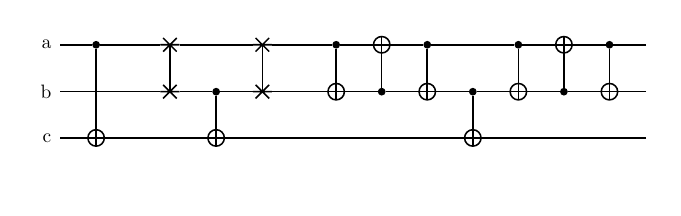
\begin{tikzpicture}
\node[scale=0.7] {
  \begin{quantikz}
  \lstick{a} & \ctrl{2} & \qw \qceq & \swap{1} & \qw & \swap{1} & \qw\qceq & \ctrl{1} & \targ{} & \ctrl{1} & \qw &\ctrl{1} & \targ{} & \ctrl{1} & \qw \\
  \lstick{b} & \qw & \qw & \swap{} & \ctrl{1} & \swap{} & \qw & \targ{} & \ctrl{-1}& \targ{} & \ctrl{1} & \targ{} & \ctrl{-1}& \targ{} & \qw \\
  \lstick{c} & \targ{} & \qw  & \qw & \targ{} & \qw & \qw & \qw & \qw & \qw & \targ & \qw & \qw & \qw & \qw  & \qw \\
  \end{quantikz}
};
\end{tikzpicture}
  \caption{Applying a CNOT gate on $(a, c)$ using a SWAP gate}
\end{figure}

\begin{figure}[h]
  \label{fig:bridge-one-with-bridge}
  \centering
  \begin{quantikz}
  \lstick{a} & \ctrl{2} & \qw \qceq & \qw & \ctrl{1} & \qw & \ctrl{1} & \qw \\
  \lstick{b} & \qw & \qw & \ctrl{1} & \targ{} & \ctrl{1}  & \targ{} & \qw \\
  \lstick{c} & \targ{} & \qw & \targ{} & \qw  & \targ & \qw  & \qw &  \qw \\
  \end{quantikz}
  \caption{Applying a CNOT gate on $(a, c)$ using a bridge gate}
\end{figure}

Figure~\ref{fig:bridge-one-with-swap} and \ref{fig:bridge-one-with-bridge} show the difference between using a SWAP gate and a bridge gate to perform a CNOT gate for the case of three qubits. The bridge gate is more efficient in terms of the number of CNOT gates, but it is less efficient in terms of depth.

Now, the generalized bridge gate is defined as follows~\cite{nash2020}:

\begin{definition}{Generalized Bridge Gate}
  A CNOT between qubit $1$ and $n$ can be performed using a generalized bridge gate as follows:
  \begin{equation} \mathrm{Bridge}(1, n) = \prod_{i=1}^{n - 1}(\mathrm{CNOT}(i + 1, i) \prod_{i=n - 2}^{2}\mathrm{CNOT}(i + 1, i))^2
  \end{equation}
\end{definition}


\def\qceq{\midstick[6,brackets=none]{=}}
\begin{figure}[h]
  \centering
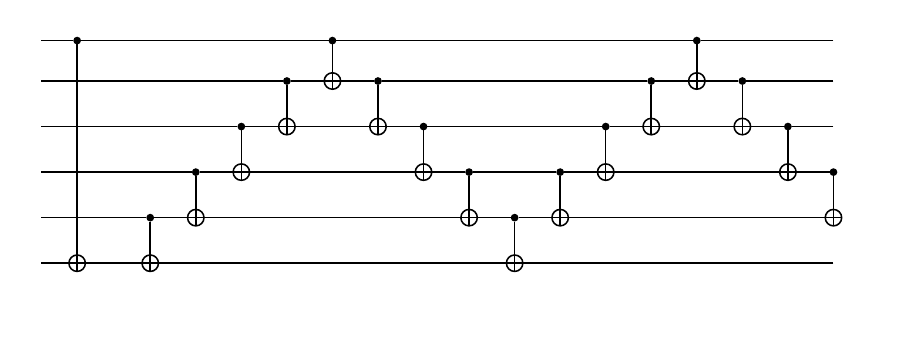
\begin{tikzpicture}
\node[scale=0.7] {
\begin{quantikz}
\qw &\ctrl{5}&\qw\qceq&
 \qw    &\qw     &\qw     &\qw     &\ctrl{1}& \qw    & \qw    & \qw     &
 \qw    &\qw     &\qw     &\qw     &\ctrl{1}& \qw    & \qw    & \qw     & \\
\qw & \qw    & \qw    &
 \qw    &\qw     &\qw     &\ctrl{1}& \targ{}&\ctrl{1}& \qw    & \qw     &
 \qw    &\qw     &\qw     &\ctrl{1}& \targ{}&\ctrl{1}& \qw    & \qw     & \\
\qw & \qw    & \qw    &
 \qw    &\qw     &\ctrl{1}& \targ{}& \qw    &\targ{} &\ctrl{1}& \qw     &
 \qw    &\qw     &\ctrl{1}& \targ{}& \qw    &\targ{} &\ctrl{1}& \qw     & \\
\qw & \qw    & \qw    &
 \qw    &\ctrl{1}&\targ{} & \qw    & \qw    & \qw    &\targ{} &\ctrl{1} &
 \qw    &\ctrl{1}&\targ{} & \qw    & \qw    & \qw    &\targ{} &\ctrl{1} & \\
\qw & \qw    & \qw    &
\ctrl{1}&\targ{} &\qw     & \qw    & \qw    & \qw    & \qw    &\targ{}  &
\ctrl{1}&\targ{} &\qw     & \qw    & \qw    & \qw    & \qw    &\targ{}  & \\
\qw &\targ{} & \qw    &
\targ{} & \qw    & \qw    & \qw    & \qw    & \qw    & \qw     & \qw    &
\targ{} & \qw    & \qw    & \qw    & \qw    & \qw    & \qw     & \qw    & \\
\end{quantikz}
};
\end{tikzpicture}
  \caption{The bridge gate for $n=6$}
\end{figure}


\chapter{Discussion}\label{chap:discussion}

\section{Problem Statement}

We have already reviewed the main research themes around quantum compilation in Chapter~\ref{chap:background}. We have seen that one of the main challenges is in imposing connectivity constraints on the circuit. Furthermore, because of the huge dependence of most of the research on swapping qubits, putting together with the fact that swapping is the most expensive two-qubit gate, it is important to study the alternatives for swapping. In this chapter, we introduce our research problem based on the definition of bridging that we discussed earlier.

While our aim in the most broad term is to find alternatives to SWAP gate, to apply gates with respect to connectivity constraints, we start with a more specific problem. We seek for optimal bridged gate, and by optimal we mean both the least number of CNOTs and the least depth. Note that, this problem is going to be studied for an arbitrary connectivity constraint $G$.

The relation of this problem to the approach of \cite{nash2020,kissinger2019} is that we are looking for bridged gates that can be adopted in the any compilation process, in contrast to theirs that is defining a whole new compilation process. In terms of the results, while some of our preliminary results such as a simple bridged CNOT gate can be derived from their techniques too, however, the main contribution of our work is to show the optimal bridged gate for any two-qubit gate, while those efforts are limited to compiling the gates that are combination of CNOTs and $R_z$s.

\section{Two-qubit Gate Classes}

Our discussion heavily relies on the KAK decomposition of two-qubit gates. We have already introduced it in Lemma~\ref{lem:kak_decomposition}. Here we introduce a few classes of two-qubit gates, based on their KAK decomposition.

\begin{definition}[Two-qubit Gate Classes]
  Based on the KAK decomposition of two-qubit gates, that is 
  \begin{equation}
    U = (V_1 \otimes V_2) e^{i \alpha X \otimes X + i \beta Y \otimes Y + i \gamma Z \otimes Z} (V_3 \otimes V_4),
  \end{equation}
  we define the following classes of two-qubit gates:
  \begin{itemize}
    \item \textbf{Class nil}: Two-qubit gates that $\alpha = \beta = \gamma = 0$.
    \item \textbf{Class I:} Two-qubit gates that only one of $\alpha, \beta, \gamma \neq 0$.
    \item \textbf{Class II:} Two-qubit gates that at least two of $\alpha, \beta, \gamma \neq 0$.
  \end{itemize}
\end{definition}

The gates in class nil are local gates that are applied on each qubit separately, so they are irrelevant to our discussion about bridging. The gates in class I, such as CNOT, CZ and etc., can be decomposed to one $\mathrm{C}R_x$ gate upto local gates. This fact is shown in Lemma~\ref{lem:crx-decomposition} and enables us to bridge them.

\begin{lemma}\label{lem:crx-decomposition}
  For any two-qubit gate $U$ in class I, it can be decomposed as 
  \begin{equation}
    U = W_1 \otimes W_2 \mathrm{C}R_x(\theta) W_3 \otimes W_4,
  \end{equation}
  where $\mathrm{C}R_x(\theta)$ is a controlled rotation gate around $x$ axis, with control on the first qubit and target on the second qubit.
\end{lemma}
\begin{proof}
  Without lose of generality, we can assume that $\gamma \neq 0$ and $\alpha = \alpha = 0$. Now, we can write
  \begin{equation}
    U = (V_1 \otimes V_2) e^{i \gamma Z \otimes Z} (V_3 \otimes V_4).
  \end{equation}
  Then, similar to the way that we derive $\mathrm{C}Z$ and $\mathrm{CNOT}$ gates, we can write
  \begin{equation}
    \begin{aligned}
    U &= (V_1 \otimes V_2 R_z(-2\gamma)) CR_z(4\theta) (V_3 \otimes V_4), \\
    &= (V_1 \otimes V_2 R_z(-2\gamma) H) CR_x(4\theta) (V_3 \otimes H V_4).
    \end{aligned}
  \end{equation}
  Now we $W_i$s are easily derived from $V_i$s.
\end{proof}

The gates in class II, such as SWAP, cannot be bridged any better than the baseline implementation mentioned in Corollary~\ref{cor:baseline-bridged}. This fact is shown later using an special trait of these gates in Lemma~\ref{lem:no-trivial-commutation}. 

\section{Bridged Gates}

Here we introduce the bridged $T$ gate for any $T$ that belongs to class I. This gate is shown under a linear connectivity constraints, so it can be used for any other connectivity constraint (by using the connecting path between the qubits). An example of this gate (bridging over $4$ qubits) is shown in Figure~\ref{fig:bridged-class-i}. Note that $V_i$s and $\theta$ can be computed using Lemma~\ref{lem:crx-decomposition}

\begin{figure}[h!]
  \label{fig:bridged-class-i}
  \centering
  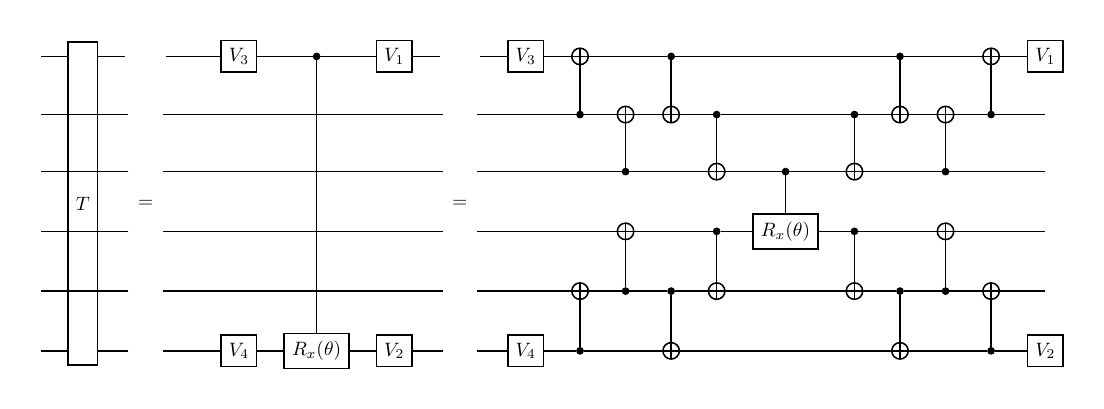
\begin{tikzpicture}
    \node[scale=0.7] {
\begin{quantikz}[transparent]
  \qw &\gate[6]{T}                        &\qw\midstick[6,brackets=none]{=}&
  \qw &\gate{V_3} & \ctrl{5} & \gate{V_1} &\qw\midstick[6,brackets=none]{=}&
  \gate{V_3} & \targ{}  & \qw     &\ctrl{1}& \qw    & \qw    & \qw    &\ctrl{1}& \qw     &\targ{}&\gate{V_1}\\
  \qw &\linethrough &\qw &
  \qw &\qw &\qw &\qw &\qw &
  \qw & \ctrl{-1}&\targ{}  & \targ{}&\ctrl{1}& \qw    &\ctrl{1}&\targ{} &\targ{}  &\ctrl{-1}&\qw\\
  \qw &\linethrough &\qw &
  \qw &\qw &\qw &\qw &\qw &
  \qw & \qw &\ctrl{-1}& \qw    & \targ{}&\ctrl{1}&\targ{} & \qw    &\ctrl{-1}&\qw & \qw \\
  \qw &\linethrough &\qw &
  \qw &\qw &\qw &\qw &\qw &
  \qw & \qw &\targ{}  & \qw    &\ctrl{1}& \gate{R_x(\theta)}&\ctrl{1}& \qw    &\targ{}  &\qw & \qw\\
  \qw &\linethrough &\qw &
  \qw &\qw &\qw &\qw &\qw &
  \qw & \targ{}  &\ctrl{-1}&\ctrl{1}& \targ{}& \qw    &\targ{} &\ctrl{1}&\ctrl{-1}&\targ{}&\qw \\
  \qw &  & \qw &
  \qw &\gate{V_4} & \gate{R_x(\theta)} & \gate{V_2} & \qw&
  \gate{V_4} & \ctrl{-1}& \qw     & \targ{}& \qw    & \qw    & \qw    &\targ{} & \qw     &\ctrl{-1}& \gate{V_2} 
  \end{quantikz}
  };
  \end{tikzpicture}
  \caption{A bridged class I gate over 6 qubits}
\end{figure}
  
This circuit above can be mathematically defined as follows:

\begin{theorem}[Bridged class I gate]
  For any class I two-qubit gate $T$, A bridged $T$ gate defined on qubits $1, n \in V$, where every $(i, i + 1) \in E$, can be implemented by the following sequence of gates:
  \begin{equation}
    T = (V_1 \otimes V_2) B^\dagger_n \mathrm{C}R_x^{\lceil n/2 \rceil \to \lceil n/2\rceil+1}(\theta) B_n (V_3 \otimes V_4),
  \end{equation}
  where $V_i$s and $\theta$ are defined in Lemma~\ref{lem:crx-decomposition}, and $B_n$ for $n = 4$ is defined as follows:
  \begin{equation}
    B_4 = (\CNOT^{1 \to 2} \otimes \CNOT^{3 \to 4}) (\CNOT^{2 \to 1} \otimes \CNOT^{4 \to 3}),
  \end{equation}
  and for an even $n \ge 6$ it could be written as follows:
  \begin{equation}
    \begin{aligned}
    B_{n} = &(\CNOT^{n/2 - 1 \to n/2} \otimes \CNOT^{n/2 + 1 \to n/2 + 2}) \\
    &(\CNOT^{n/2 - 2 \to n/2 - 1} \otimes \CNOT^{n/2 + 2 \to n/2 + 3}) \\
    &\prod_{i=1}^{n/2 - 3} (\CNOT^{i \to i+1} \otimes \CNOT^{i+3 \to i+2} \otimes \CNOT^{n-i-1 \to n-i-2} \otimes \CNOT^{n-i \to n-i+1}) \\
    &(\CNOT^{3 \to 2} \otimes \CNOT^{n-1 \to n-2}) \\
    &(\CNOT^{2 \to 1} \otimes \CNOT^{n \to n-1}).
    \end{aligned}
  \end{equation}
  and, for any odd $n$ it could be recovered by removing $n$th qubit and its corresponding CNOTs from $B_n$.
\end{theorem}
\begin{proof}
  In order to prove the correctness of this circuit, we will show that it is equivalent to the baseline implementation of bridged $T$ gate (Corollary~\ref{cor:baseline-bridged}).
  
  First, using the fact that $[\CNOT^{i \to j}, \CNOT{i \to k}] = 0$ and $[\CNOT^{i \to j}, \CNOT^{k \to j}] = 0$, we can show that $B_n$ (for even $n$) could be rearranged as:

  \begin{equation}
    B_n = \prod_{i=1}^{n/2 - 1} (\CNOT^{i\to i+1}\CNOT{i+1\to i}) \otimes (\CNOT^{n-i\to n-i+1} \CNOT{n-i+1\to n-i}).
  \end{equation}

  This rearrangement for $n = 6$ is shown in Figure~\ref{fig:bridged-class-i-proof-a}.

  \begin{figure}[h!]
    \label{fig:bridged-class-i-proof-a}
    \centering
    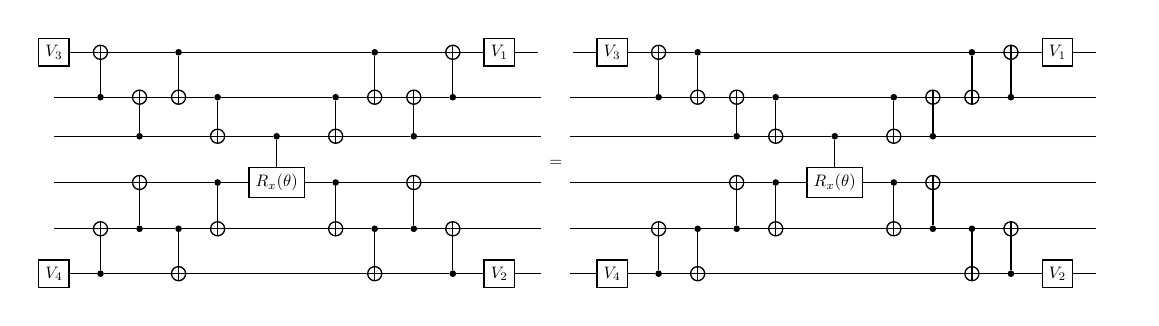
\begin{tikzpicture}
      \node[scale=0.6] {
  \begin{quantikz}[transparent]
    \gate{V_3} & \targ{}  & \qw     &\ctrl{1}& \qw    & \qw    & \qw    &\ctrl{1}& \qw     &\targ{}&\gate{V_1}&\qw\midstick[6,brackets=none]{=}&
    \gate{V_3} & \targ{}  &\ctrl{1}& \qw     & \qw    & \qw    & \qw    & \qw     &\ctrl{1}&\targ{}&\gate{V_1}& \qw \\
    \qw & \ctrl{-1}&\targ{}  & \targ{}&\ctrl{1}& \qw    &\ctrl{1}&\targ{} &\targ{}  &\ctrl{-1}&\qw&\qw&
    \qw & \ctrl{-1}&\targ{}  & \targ{}&\ctrl{1}& \qw    &\ctrl{1}&\targ{} &\targ{}  &\ctrl{-1}&\qw&\qw\\
    \qw & \qw &\ctrl{-1}& \qw    & \targ{}&\ctrl{1}&\targ{} & \qw    &\ctrl{-1}&\qw & \qw & \qw &
    \qw & \qw & \qw    &\ctrl{-1}& \targ{}&\ctrl{1}&\targ{} &\ctrl{-1}& \qw    &\qw & \qw & \qw \\
    \qw & \qw &\targ{}  & \qw    &\ctrl{1}& \gate{R_x(\theta)}&\ctrl{1}& \qw    &\targ{}  &\qw & \qw&\qw&
    \qw & \qw   & \qw    &\targ{}&\ctrl{1}& \gate{R_x(\theta)}&\ctrl{1}&\targ{}& \qw      &\qw & \qw&\qw&\\
    \qw & \targ{}  &\ctrl{-1}&\ctrl{1}& \targ{}& \qw    &\targ{} &\ctrl{1}&\ctrl{-1}&\targ{}&\qw&\qw& 
    \qw & \targ{}  &\ctrl{1}&\ctrl{-1}& \targ{}& \qw    &\targ{} &\ctrl{-1}&\ctrl{1}&\targ{}&\qw&\qw\\
    \gate{V_4} & \ctrl{-1}& \qw     & \targ{}& \qw    & \qw    & \qw    &\targ{} & \qw     &\ctrl{-1}& \gate{V_2} &\qw&
    \gate{V_4} & \ctrl{-1}& \targ{} & \qw  & \qw    & \qw    & \qw     & \qw     &\targ{}&\ctrl{-1}& \gate{V_2} &\qw&
    \end{quantikz}
    };
    \end{tikzpicture}
    \caption{Rearrangement of CNOTs that is used in the proof}
  \end{figure}

  Then, using the fact that 
  \begin{equation}
    \SWAP^{i,j} = \CNOT^{j \to i} \CNOT^{i \to j} \CNOT^{j \to i},
  \end{equation}
  it could be simplified further to
  \begin{equation}
    B_n = \prod_{i=1}^{n/2 - 1} (\CNOT^{i+1 \to i} \SWAP^{i, i+1}) \otimes (\CNOT{n-i+1\to n-i}\SWAP^{n-i, n-i+1}).
  \end{equation}

  Now, by moving the rearranging the CNOTs to be applied after the SWAPs, we will have
  \begin{equation}
    B_n = \prod_{i=1}^{n/2 - 1} \CNOT^{n/2 \to i} \otimes \CNOT^{n-i+1 \to n/2 + 1} \prod_{i=1}^{n/2 - 1} \SWAP^{i, i+1} \otimes \SWAP^{n-i, n-i+1}.
  \end{equation}

  This process is shown in Figure~\ref{fig:bridged-class-i-proof-b} for $n = 6$.
  
  \begin{figure}[h!]
    \label{fig:bridged-class-i-proof-b}
    \centering
    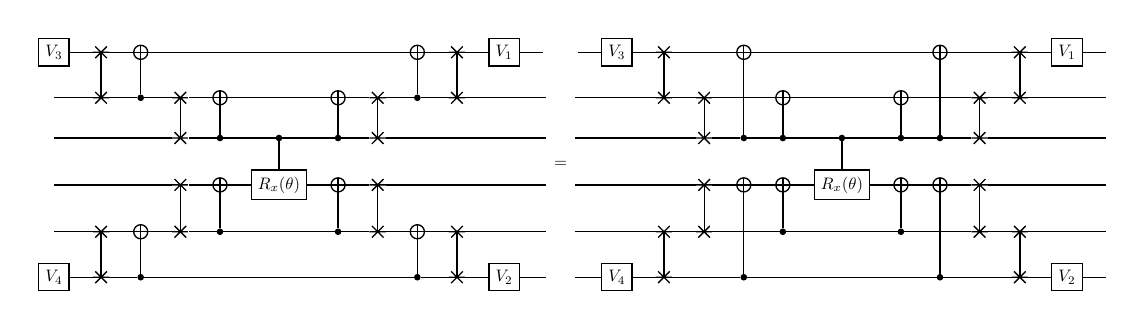
\begin{tikzpicture}
      \node[scale=0.6] {
  \begin{quantikz}[transparent]
    \gate{V_3} & \swap{}  &\targ{}& \qw     & \qw    & \qw    & \qw    & \qw     &\targ{}&\swap{}&\gate{V_1}&\qw\midstick[6,brackets=none]{=}&
    \gate{V_3} & \swap{}  & \qw     &\targ{}& \qw    & \qw    & \qw    &\targ{}& \qw     &\swap{}&\gate{V_1}&\qw \\
    \qw & \swap{-1}&\ctrl{-1}  & \swap{}&\targ{}& \qw    &\targ{}&\swap{} &\ctrl{-1}  &\swap{-1}&\qw&\qw&
    \qw & \swap{-1}& \swap{}&\qw&\targ{}& \qw    &\targ{}&\qw &\swap{} &\swap{-1}&\qw&\qw\\
    \qw & \qw & \qw    &\swap{-1}& \ctrl{-1}&\ctrl{1}&\ctrl{-1} &\swap{-1}& \qw    &\qw & \qw & \qw &
    \qw & \qw &\swap{-1}& \ctrl{-2} & \ctrl{-1}&\ctrl{1}&\ctrl{-1} &\ctrl{-2}& \swap{-1}    &\qw & \qw & \qw\\
    \qw & \qw   & \qw    &\swap{1}&\targ{}& \gate{R_x(\theta)}&\targ{}&\swap{1}& \qw      &\qw & \qw&\qw&
    \qw & \qw   & \swap{1}    &\targ{}&\targ{}& \gate{R_x(\theta)}&\targ{}&\targ{}& \swap{1}      &\qw & \qw&\qw\\
    \qw & \swap{1}  &\targ{}&\swap{}& \ctrl{-1}& \qw    &\ctrl{-1} &\swap{}&\targ{}&\swap{1}&\qw&\qw& 
    \qw & \swap{1}  &\swap{}&\qw& \ctrl{-1}& \qw    &\ctrl{-1} &\qw&\swap{}&\swap{1}&\qw&\qw\\
    \gate{V_4} & \swap{}& \ctrl{-1} & \qw  & \qw    & \qw    & \qw     & \qw     &\ctrl{-1}&\swap{}& \gate{V_2} &\qw&
    \gate{V_4} & \swap{}&  \qw & \ctrl{-2} & \qw    & \qw    & \qw     &\ctrl{-2}& \qw     &\swap{}& \gate{V_2} &\qw
    \end{quantikz}
    };
    \end{tikzpicture}
    \caption{Moving CNOTs across the SWAPs that is used in the proof}
  \end{figure}

  Finally, the second product term is similar to the one in Corollary~\ref{cor:baseline-bridged}, and the first product term is a sequence of CNOTs that all commute with $\mathrm{C}R_x^{n/2 \to n/2 + 1}(\theta)$, so they will be canceled in $B_n^\dagger \mathrm{C}R_x^{n/2 \to n/2 + 1}(\theta) B_n$.

  \begin{equation}
    \begin{aligned}
    B^\dagger_n \mathrm{C}R_x^{n/2 \to n/2 + 1}(\theta) B_n &= \prod_{i=n/2 - 1}^{1} \SWAP^{i, i+1} \otimes \SWAP^{n-i, n-i+1} \\
    & \phantom{=}~\mathrm{C}R_x^{n/2 \to n/2 + 1}(\theta) \\
    & \phantom{=}~\prod_{i=1}^{n/2 - 1} \SWAP^{i, i+1} \otimes \SWAP^{n-i, n-i+1} \\
    &= \mathrm{C}R_x^{1 \to n}(\theta)
    \end{aligned}
  \end{equation}

  Finally, by recalling Lemma~\ref{lem:crx-decomposition},
  \begin{equation}
    (V_1 \otimes V_2) B^\dagger_n \mathrm{C}R_x^{\lceil n/2 \rceil \to \lceil n/2\rceil+1}(\theta) B_n (V_3 \otimes V_4) = T.
  \end{equation}
  
  In order to prove the correctness of the circuit for odd $n$ as well, we can simply remove the $n$th qubit and its corresponding CNOTs from $B_n$. This fact will be propagated through the proof and every other thing will be the same.
\end{proof}

The formula above shows that the circuit uses $4n + O(1)$ CNOTs with the depth $n + O(1)$ (noting that $\mathrm{C}R_x$ needs two CNOTs \cite[chapter 4]{nielsen2010}). 
While in comparison to the baseline implementation (see Corollary~\ref{cor:baseline-bridged}), this circuit has $33\%$ improvement in the number of CNOTs and $66\%$ improvement in the depth. Even for the special case of CNOT, this circuit has approximately the same number of CNOTs as the bridged CNOT gate in Equation~\ref{eq:bridged-cnot-m-n} and Figure~\ref{fig:bridged-cnot-m-n}, however, its depth is improved by $75\%$.

\section{Proof of Optimality}

Here we aim to proof the optimality of the bridged $T$ gate described in the previous section for class I gates, and the baseline implementation for class II gates. By optimality we mean that the number of CNOTs and the depth of the circuit is the minimum possible (upto an $O(1)$ constant).

We start by introducing the the tools and the intuition behind their definitions, in addition to the core lemma that is used in the proofs. Then, we will prove the results for class I and class II gates separately. The first tool that we need is conjugation that is commonly used in group theory \cite{weisstein}.

\begin{definition}[Conjugation]
  For any two gates $A$ and $B$, we define the conjugation of $A$ by $B$ as
  \begin{equation}
    B^\dagger A B.
  \end{equation}
\end{definition}

The intuition behind the conjugation of gates is that if the conjugation of $A$ by $B$ is $C$, then applying $A$ before $A$ is equivalent to applying $C$ after $B$. Informally this could be phrased as by crossing $A$ over $B$, $A$ will be transformed to $C$. Figure~\ref{fig:conjugations} shows a few conjugations that we will use in the proofs.

\begin{figure}[ht]\label{fig:conjugations}
  \centering
  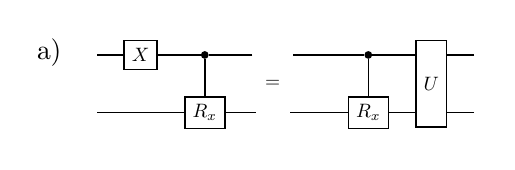
\begin{tikzpicture}
    \node at (-3, 0.4) {a)};
    \node[scale=0.7] {\begin{quantikz}
    \qw & \gate{X} & \ctrl{1} & \qw\midstick[2,brackets=none]{=} & \qw & \ctrl{1} & \gate[2]{U} & \qw \\
    \qw & \qw & \gate{R_x} & \qw & \qw & \gate{R_x} & \qw & \qw 
  \end{quantikz}};\end{tikzpicture} \\
  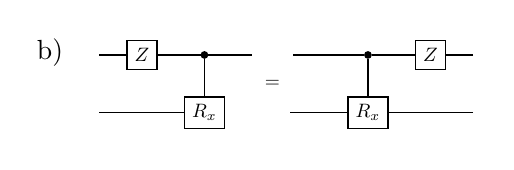
\begin{tikzpicture}
    \node at (-3, 0.4) {b)};
    \node[scale=0.7] {\begin{quantikz}
    \qw & \gate{Z} & \ctrl{1} & \qw\midstick[2,brackets=none]{=} & \qw & \ctrl{1} & \gate{Z} & \qw \\
    \qw & \qw & \gate{R_x} &  & \qw & \gate{R_x} & \qw & \qw 
  \end{quantikz}};\end{tikzpicture} \\
  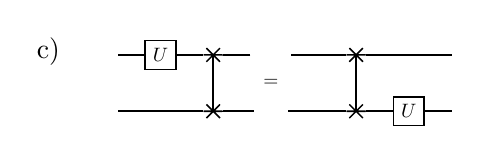
\begin{tikzpicture}
    \node at (-3, 0.4) {c)};
    \node[scale=0.7] {\begin{quantikz}
    \qw & \gate{U} & \swap{1} & \qw\midstick[2,brackets=none]{=} & \qw & \swap{1} & \qw &  \qw \\
    \qw & \qw & \swap{} & \qw & \qw & \swap{} & \gate{U} & \qw 
  \end{quantikz}};\end{tikzpicture}
  \caption{a) Conjugation of $X \otimes I$ by $\mathrm{C}R_x$ is a two-qubit gate. b) Conjugation of $Z \otimes I$ by $\mathrm{C}R_x$ is $Z \otimes I$. c) Conjugation of $U \otimes I$ by SWAP is $I \otimes U$}.
\end{figure}

Furthermore, this effect, will help us to develop a tool to properly analyse the flow of information in a circuit. To complete this idea we define a sense of locality, using the following simple definition:

\begin{definition}[Trivial/Nontrivial action]
  A gate $U$ defined on a set of qubits $Q$ is acting trivially on qubit $q \in Q$ if $U$ can be written as 
  \begin{equation}
    U = U' \otimes I_q
  \end{equation}
  where $U'$ is a gate defined on $Q \setminus \{ q \}$ and $I_q$ is the identity gate on qubit $q$.
  Respectively, $U$ is acting nontrivially on $q$ if it cannot be written in the above form.
\end{definition}

Now, these proofs are based on the idea that if two gate sequence $A = A_n \dots A_2 A_1$ and $B = B_m \dots B_2 B_1$ are equal, then the conjugation of any arbitrary gate $U$ by $A$ is equal to the conjugation of $U$ by $B$. Or in another word,

\begin{corollary}
  Assume $A = A_n \dots A_2 A_1$ and $B = B_m \dots B_2 B_1$ are two gate sequences, then the necessary condition for $A = B$ is that for any arbitrary gate $U$, the conjugation of $U$ by $A$ must be equal to the conjugation of $U$ by $B$.
\end{corollary}

This corollary will be amazingly useful by noting the fact that the conjugation of $U$ by $A$ can be iteratively computed as follows:

\begin{equation}
  \begin{cases}
    U_1 = \text{conjugation of } U \text{ by } A_1 \\
    U_{i+1} = \text{conjugation of } U_i \text{ by } A_{i+1}
  \end{cases}
  \Rightarrow U_n = \text{conjugation of } U \text{ by } A.
\end{equation}

Now, we can start proving the optimality of the bridged $T$ gate for different classes, starting by class I.

\subsection{Class I}

The sketch of this proof consists of first reducing the problem to bridging a $\mathrm{C}R_x^{1\to n}$ gate. Then because of the nontrivial (on $1$ and $n$) conjugations of $X_1$ and $Z_n$ by $\mathrm{C}R_x^{1\to n}$, we can conclude that any sequence of gates that is bridged $\mathrm{C}R_x^{1\to n}$ needs to have a minimum number of CNOTs, and a minimum depth, to produce such nontrivial conjugations. These two bounds are achieved by the bridged $T$ gate.

So, to start the proof, we first establish two facts about the conjugations:
\begin{corollary}[No-go for one-qubit gates]\label{cor:no-go-one-qubit}
  For any gate acting trivially on $t$, its conjugation by any one-qubit gate on $t$ is still trivial on $t$. 
\end{corollary}

This corollary informally states that if we want to create nontrivial action on $t$ by conjugation, we need use two-qubit gates. This fact can be easily shown by simply combining definition of trivial action and conjugation.

\begin{lemma}[No-move for class I gates]\label{lem:no-move-class-i}
  For any gate $A$ acting nontrivially on $n$ and trivially on $t$, its conjugation $B$ by any class I gate $U$ acting on $n$ and $t$, is nontrivial on $n$.
\end{lemma}
\begin{proof}
  Noting that $A$ must be trivial on $t$ and nontrivial on $n$, $A$ could be decomposed as $A' \otimes I_t$.
  Using the definition of conjugation in form of $U^\dagger A U = B$, we can write

  \begin{equation}
    \begin{aligned}
    B &= U^\dagger (A' \otimes I_t) U  \\
    &= (V_3^\dagger \otimes V_4^\dagger)\mathrm{C}R_x(-\theta) (V_1^\dagger A' V_1 \otimes I) \mathrm{C}R_x(\theta) (V_3 \otimes V_4) \\
    &= (V_3^\dagger \otimes V_4^\dagger)(\dyad{0} + R_x(-\theta) \otimes \dyad{1}) (V_1^\dagger A' V_1 \otimes I) (\dyad{0} + R_x(\theta) \otimes \dyad{1}) (V_3 \otimes V_4) \\
    &= (V_3^\dagger \otimes V_4^\dagger)(V_1^\dagger A' V_1 \dyad{0} + R_x(-\theta) V_1^\dagger A' V_1 R_x(\theta) \dyad{1}) (V_3 \otimes V_4)
    \end{aligned}
  \end{equation}

  We have used the decomposition of Lemma~\ref{lem:crx-decomposition} for $U$ and expanded $\mathrm{C}R_x$ in terms of $\dyad{0}$ and $\dyad{1}$. Then, in order to proof by contradiction, we can assume that $B = I_n \otimes B'$, then $\tr_n(B) = B'$, so
  \begin{equation}
    B' = \tr_n(B) = \tr_n(A') \dyad{0}_n + \tr_n(A') \dyad{1}_n = \tr_n(A') I_t
  \end{equation}
  which means that $B = \tr_n(A') \otimes I_n \otimes I_t$, that results in $A = \tr_n(A') \otimes I_n \otimes I_t$,  as well. Which is a contradiction with the assumption that $A$ is nontrivial on $n$.
\end{proof}

Now, we can prove the optimality of the bridged $T$ gate for class I gates in the theorem below.

\begin{theorem}\label{thm:no-go-class-i}
  Any bridged $T$ gate where $T$ is a class I gate acting on qubits $1$ and $n$ with linear connectivity, needs at least $4n + O(1)$ CNOTs and has at least $n$ depth.
\end{theorem}
\begin{proof}
  Without losing generality, we can assume that $T = \mathrm{C}R_x^{1\to n}(\theta)$, because of Lemma~\ref{lem:crx-decomposition}. We can also show that the conjugation of $X_1$ and $Z_n$ (one qubit gates acting on qubits $1$ and $n$ respectively) by $T$ is nontrivial on $1$ and $n$ Then, we assume that a sequence of gates $A = A_\ell \dots A_2 A_1$ is equivalent to $T$, 
  the conjugation of $X_1$ and $Z_n$ under $A$ must be nontrivial on $1$ and $n$ as well. 

  In order to simplify the notation, we name the conjugation of $X_1$ and $Z_n$ by $A_i \dots A_1$ as $\xi_i$ and $\zeta_i$ respectively. Now, based on the fact that one-qubit gates could not create nontrivial action (Corollary~\ref{cor:no-go-one-qubit}), and because of the connectivity constraint, in order to have nontrivial action on $n$ by $\xi_n$, we need to a CNOT gate acting on $n$ and $n-1$, or in another word $A_j = \CNOT^{n \rightleftharpoons n-1}$ for some $j \le \ell$. Also $\xi_{j - 1}$, must act nontrivially on $n-1$. Moreover, using Lemma~\ref{lem:no-move-class-i} we know that using one CNOT ($A_j$) will leave $\xi_{j}$ acting nontrivially on $n-1$, which is not desired. This means that at least two CNOTs are necessary, or in another word $A_k = \CNOT^{n-1 \rightleftharpoons n-1 \pm 1}$ for $j < k \le \ell$. By recursively applying this argument, we can conclude that a sequence of CNOT pairs acting on subsequent qubits from $1$ to $n$ is necessary solely to make $\xi_n$ to have nontrivial action on $n$. A similar argument could hold for $\zeta_n$. Now because of the fact that these two sequences are going in opposite directions, and they cannot have more than $O(1)$ gates in common, we can conclude that at least $4(n-1) + O(1)$ CNOTs are necessary to have nontrivial action on $1$ and $n$ by $\xi_n$ and $\zeta_n$. Note that the minimum depth could be easily derived from the fact that a CNOT between $n$ and $n-1$ should take place after a CNOT between $n-1$ and $n-2$ and so on.
\end{proof}

\subsection{Class II}

For the class II, we will prove in a similar manner that there is no solution better than the baseline implementation (Corollary~\ref{cor:baseline-bridged}). Here we start by a lemma that shows the distinctive feature of the class II gates to be used in the proof.

\begin{lemma}\label{lem:no-trivial-commutation}
  for any gate $A$ acting nontrivially on $n$ and trivially on $t$, its conjugation $B$ by a class II gate $U$ acting on $n$ and $t$, is nontrivial on $t$. 
\end{lemma}
\begin{proof}
  Similar to the approach in proving Lemma~\ref{lem:no-move-class-i}, using proof by contradiction, we can assume that $B = B' \otimes I_t$, then
  \begin{equation}
    \begin{aligned}
      (A' \otimes I_t) U  &= U (B' \otimes I_t) \\
      (A' V_1 \otimes V_2) e^{i \alpha X \otimes X + i \beta Y \otimes Y + i \gamma Z \otimes Z} (V_3 \otimes V_4) &= (V_1 \otimes V_2) e^{i \alpha X \otimes X + i \beta Y \otimes Y + i \gamma Z \otimes Z} (V_3 B' \otimes V_4). 
    \end{aligned}
  \end{equation}
  Then by multiplying $(V_1^\dagger \otimes V_2^\dagger)$ from left and $(V_3^\dagger \otimes V_4^\dagger)$ from right, we can write
  \begin{equation}
      (V_1^\dagger A' V_1 \otimes I_t) e^{i \alpha X \otimes X + i \beta Y \otimes Y + i \gamma Z \otimes Z} = e^{i \alpha X \otimes X + i \beta Y \otimes Y + i \gamma Z \otimes Z} (V_3 B' V_3^\dagger \otimes I_t).
  \end{equation}

  Now, by expanding the exponential, we will have
  \begin{equation}
    \begin{aligned}
      (V_1^\dagger A' V_1 \otimes I_t) & (c_1 I \otimes I + i c_2 X \otimes X + i c_3 Y \otimes Y + i c_4 Z \otimes Z) \\
      = &(c_1 I \otimes I + i c_2 X \otimes X + i c_3 Y \otimes Y + i c_4 Z \otimes Z) (V_3 B' V_3^\dagger \otimes I_t).  
    \end{aligned}
  \end{equation}
  Where $c_i$s are some constants. Finally, by multiplying both sides by $(I_n \otimes P)$ where $P$ is one of $I, X, Y, Z$, and then by tracing out the qubit $t$, we will have the following equations:
  \begin{equation}
    \begin{cases}
      V_1^\dagger A' V_1 = V_3 B' V_3^\dagger \\
      V_1^\dagger A' V_1 X = X V_3 B' V_3^\dagger & \text{if }\alpha \ne 0 \\
      V_1^\dagger A' V_1 Y = Y V_3 B' V_3^\dagger & \text{if }\beta \ne 0 \\
      V_1^\dagger A' V_1 Z = Z V_3 B' V_3^\dagger & \text{if }\gamma \ne 0. \\
    \end{cases}
  \end{equation}

  It means that if two of $\alpha, \beta, \gamma$ are non-zero, then $A$ must have the form $A' = A'' \otimes I_n$ which is against the assumption that $A$ is nontrivial on $n$.
\end{proof}

Now, we can prove the main theorem.

\begin{theorem}\label{thm:no-go-class-ii}
  Any bridged gate where $T$ is a class II gate acting on qubits $1$ and $n$ with linear connectivity, needs at least $6n + O(1)$ CNOTs and has at least $3n$ depth.
\end{theorem}
\begin{proof}
  This proof is similar to the proof of Theorem~\ref{thm:no-go-class-i}, 
  assume that $A_j = \CNOT^{1 \to 2}$ is the only CNOT applying on qubits $1$ and $2$. We have assumed the direction without loose of generality as the other direction could be proved similarly. Now, the conjugation of $Z_1$ (acting on qubit $1$) by $A^\dagger_1 \dots A^\dagger_{j-1}$ that we call it $U_1$ must be nontrivial on qubit $1$. Using Lemma~\ref{lem:no-trivial-commutation}, the conjugation of $U_1$ by $T$ must act nontrivial on $n$. On the other hand the conjugation of $U_1$ under $A_j\dots A_1$ is equal to the conjugation of $Z_1$ under $A_j$ which is trivial on $2$ and will be trivial on any $i \ge 2$ as $A_j$ is the only CNOT between $1$ and $2$, which is not compatible with the assumption of acting nontrivially on $n$. This means that at least two CNOTs are necessary. We call the second CNOT as $A_k$ where $j < k$. Now, using Lemma~\ref{lem:no-move-class-i} we know that the conjugation of $U_1$ by $A_k\dots A_1$ is still nontrivial on $2$ that is not desired, so the third CNOT is necessary as well. Recursively we can conclude that a sequence made of three CNOTs is necessary. All of these arguments could be applied in the other direction, so we can conclude that at least $6n + O(1)$ CNOTs are necessary. 
\end{proof}
\subsection{Extension to Arbitrary Connectivity}

The extension to arbitrary connectivity is can be done by defining layers. Layers are used to linearizing the vertices of the graph with respect to their distance from a node. Then, the proof of Theorem~\ref{thm:no-go-class-i} and Theorem~\ref{thm:no-go-class-ii}
% TODO
 Given a connectivity graph $G = (V, E)$, and a target gate $T$ that is defined on $a,b \in V$, we can define a set of layers $L_1 \dots L_k$, defined as
\begin{equation}
  L_i = \{ v \in V \mid \mathrm{dist}(v, a) = i \}.
\end{equation}
Where $\mathrm{dist}(v, a)$ is the distance between $v$ and $a$ in $G$. Then, the whole proof could be re used, with the only difference that instead of acting nontrivially on $i$th qubit, now we care about acting nontrivially on one of the qubits in $L_i$. This means that the number of CNOTs and the depth will be $4\mathrm{dist}(a,b) + O(1)$ and $\mathrm{dist}(a,b) + O(1)$ respectively. 

% TODO more formal things
% TODO some shapes (for layers)

\chapter{Implementation}\label{chap:implementation}



\chapter{Conclusion}\label{chap:conclusion}

TODO


\printbibliography

\end{document}

